
\documentclass[11pt]{article}
\usepackage{llncsdoc}
%\usepackage{natbib}
\usepackage{times}
\usepackage{url}
\usepackage{latexsym}
\usepackage{xspace}
\usepackage{multirow}
\usepackage{paralist}
\usepackage{amsmath}
\usepackage{graphicx}
\usepackage{url}
\usepackage[toc,page]{appendix}
\usepackage{amsthm}
\newtheorem{definition}{Definition}

%\eaclfinalcopy % Uncomment this line for the final submission
%Position of pdflatex: /Library/TeX/Root/bin/x86_64-darwin
%
\newcommand\BibTeX{B{\sc ib}\TeX}


\newcommand\original{\textsc{Original}\xspace}
\newcommand\twitter{\textsc{Twitter}\xspace}

\newcommand\glove{GloVe\xspace}

\newcommand{\eqnref}[1]{Equation~\ref{#1}}
\newcommand{\figref}[1]{Figure~\ref{#1}}
\newcommand{\figsref}[2]{Figures~\ref{#1} and \ref{#2}}
\newcommand{\posciteauthor}[1]{\citeauthor{#1}'s}
\newcommand{\poscite}[1]{\citeauthor{#1}'s \citeyearpar{#1}}
\newcommand{\secref}[1]{Section~\ref{#1}}
\newcommand{\secsref}[2]{Sections~\ref{#1} and \ref{#2}}
\newcommand{\sentref}[1]{(\ref{#1})}
\newcommand{\tabref}[1]{Table~\ref{#1}}
\newcommand{\tabsref}[2]{Tables~\ref{#1} and \ref{#2}}

\newcommand\dev{\textsc{dev}\xspace}
\newcommand\test{\textsc{test}\xspace}

\setlength{\textfloatsep}{3pt}

\title{Text-based Detection of Unauthorized Users of Social Media Accounts}

%\author{Milton King  \\
%Faculty of Computer Science, University of New Brunswick\\
%Fredericton, NB E3B 5A3, Canada\\
%\tt{milton.king@unb.ca}}

%To do
%Read a paper that uses OneClassSVM
%Different type of media or data that used author verification
%Cite sklearn: http://scikit-learn.org/stable/about.html#citing-scikit-learn

%\date{Nov. 27, 2017}

\begin{document}


\maketitle

\begin{abstract}
Although social media platforms can assist organizations' progress, they also make them vulnerable to unauthorized users gaining access to their account and posting as the organization. This can have negative effects on the company including the defacing of a public appearance and a decrease in profit. An issue in this scenario is that once an attacker gains access to a social media account, they are able to post any content from that account. In this paper, we propose an author verification task in the realm of blog posts to detect and block unauthorized users based on the textual content of their unauthorized post. We use different methods to represent a document, such as word frequency and word2vec, and train two different classifiers over these document representations. The experimental results show that regardless of the classifier the word2vec method outperforms other representations.


 %% We also describe how such an author verification system can be applied to a generic social media platform.

\end{abstract}

\section{Introduction}
%There have been many cases of unauthorized personnel gaining access to social media accounts and posting content posing as the true owner of the account. An inappropriate post from a social media account can cause the defacing of a public image for both an individual and organization as well as the possibility for a loss of profit for the latter. 
%Many organizations now use social media to aid in their progression and success. This however comes with the cost that any posts made by an account belonging to an organization or individual represents them regardless of who was the actual author of a post, according to the public. One instance where an unauthorized personnel gained access and posted from the social media account of an organization is a tweet sent by an account belonging to the Associated Press, which caused nearly 130 billion dollars worth of stocks to temporarily be lost~\cite{financialTimes}.  
%\begin{figure}
%\small
%\begin{center}
%  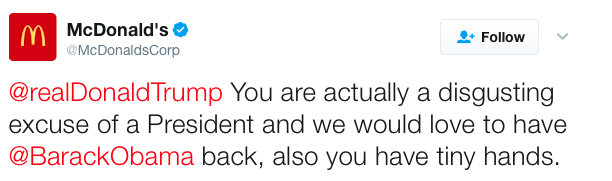
\includegraphics[width=0.66\linewidth]{./mcDonalds}
%  \caption{Tweet sent from an unauthorized user on the McDonald's Twitter account. Image taken from http://money.cnn.com/2017/03/16/ technology/mcdonalds-trump-tweet/}
%  \label{mcDonalds}
%\end{center}
%\end{figure}

Although verification by passwords are implemented to protect social media accounts, these are not completely secure. An unauthorized user can gain access to another person's or organization's social media account and publish content posing as the victim, such is the case when a post was published from Associated Press' twitter account containing the phrases \textit{Breaking: Two explosions in the White House and Barack Obama is injured}, which caused nearly 130 billion dollars worth of stocks to temporarily be lost~\cite{financialTimes}. We propose an author verification framework that predicts if a post from a social media account is written by the legitimate author or an imitator after unauthorized access to the account. This system does not stop the social media account from being accessed by an unauthorized user but rather is a form of damage control to block imitators from posting from social media accounts. We consider a variety of methods to represent documents from the original author, and train two different classifiers over these document representations to predict if a given document belongs to the authorized author or an imitator. The main contributions of our paper can be summarized as follows: $1)$ We propose an author verification framework that considers a variety of different representations of documents, and two different classifiers. $2)$ We consider a one-class SVM as an alternative to the Jankowska. $3)$ We show that representing a document via averaging word embeddings captures the style of an author and achieves the highest performance. We further show that a one-class SVM outperforms the classification approach of \cite{jankowska2014}.

%\begin{compactitem}
%    \item We propose an author verification
%framework that considers a variety of different representations of documents, and two different classifiers. The framework has the following characteristics:
%\begin{itemize}
%    \item Representing a document using the following approaches:       bag-of-words (BOW, ``word frequency'' below), BOW restricted to       only stopwords, and word embeddings~\cite{Mikolov+:2013b}.
%    \item  Extending the dissimilarity approach proposed by Jankowska \emph{et al.} ~\cite{jankowska2014} by better representing each document using word embeddings and stopword distribution and by computing the cosine distance depending on the cosine similarity.
%
%\item Considering a one-class SVM as an alternative to the Jankowska   \emph{et al.} approach.
%\end{itemize}
%
%\item We evaluate a variety of methods and classifiers using both accuracy and F-score. %(@Melton add something about the experimental experiments) Checked
%	    
%\item  We show that representing a document via averaging word embeddings captures the style of an author and achieves the highest performance. We further show that a one-class SVM outperforms the classification approach of Jankowska \emph{et al.}



%\end{compactitem}



%
%\begin{figure}
%\small
%\begin{center}
%  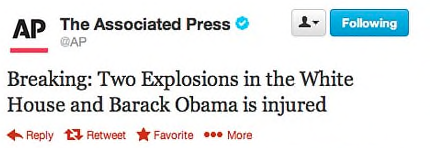
\includegraphics[width=.66\linewidth]{./associatedPress}
%  \caption{Tweet sent from an unauthorized user on the Associated
%    Press' Twitter account. Image taken from
%    http://www.telegraph.co.uk/finance/markets/10013768/Bogus-AP-tweet-about-explosion-at-the-White-House-wipes-billions-off-US-markets.html}
%  \label{press}
%\end{center}
%\end{figure}
%The rest of the paper is organized as follows. Section~\ref{litReview} presents related work. In Section~\ref{sec:overview} we
%present a general overview about the author verification framework in the domain of social media. Section~\ref{sec:representation} details the different document representations whereas Section~\ref{sec:classifiers}
%details the adopted classifiers. In Section~\ref{sec:experimentalresults} we present the experimental results.  Finally, concluding remarks and a discussion of future work are presented in Section~\ref{sec:conclusion}.


%This system will use author verification to predict if a text being published does belong to the authorized user, and if it predicts that it does not belong to the authorized user then a lockout occurs so that a secondary password is required to publish anything more from the account. 

%There have been many cases of unauthorized personnel gaining access to social media accounts and posting content posing as the true owner of the account. An inappropriate post from a social media account can cause the defacing of a public image for both an individual and organization as well as the possibility for a loss of profit for the latter. In this work, I show that word embeddings can be applied to author verification, which involves determining the true author of a text, to better protect against unauthorized users posting from a social media account. More specifically, a model that is trained on known documents --documents belonging to the authorized author-- must predict if an unknown document --document whose identity is unknown at the time-- belongs to the authorized author. In this paper, I discuss the motivation for this work, a literature review surrounding this topic, information pertaining to the experiment that includes the research plan, design component, and implementations. I finish by concluding my findings as well as discussing the direction that this work can taken such as steps to possibly better my results and other methods that can be implemented to better protect social media accounts. I also provide a demonstration on how an author verification system can be used to protect a social media account.



%[Discuss number of social media accounts hacked] 



\section{Related work} \label{litReview}
%A simple post can harm an organization \cite{oehri2012social}, whether it be from an authorized user or an unauthorized user. The insider threat in social media is when an authorized user of a social media account is responsible for harming an organization through the use of their social media account. This could be intended or accidental as in the case where an email was sent from Adidas with the title \textit{Congrats, you survived the Boston marathon!}. Some may see this as being perfectly acceptable in society, but others would associate it with the bombing that occurred at the Boston marathon in 2013. The insider threat exists in all realms of an organization where a person can harm a company from with the organization. \cite{gritzalis} evaluates personality traits of a social media user, specifically a Twitter user, to determine if they are or will become an insider threat to an organization by observing their behavior in social media. This work does not follow my work's direction but it is another method in protecting one's assets by analyzing social media. The insider threat is a serious issue for organizations, but this paper will focus on unauthorized users gaining access to a social media account.



%For example, if an author has 90\% of their emails containing 3 paragraphs then a rule can say that if a given email contains 3 paragraphs and the rule passes some threshold, then the email could belong to them. They performed rule pruning to remove rules that do not distinguish between authors well. Some of the features that were used include punctuation, n-grams, spelling errors, and rare word sequences. They used accuracy as their evaluation metric, which is the main metric that we use.

PAN\footnote{\url{http://pan.webis.de}} is an organization that releases shared tasks for researchers to work on and test their models. In 2013, PAN released an author verification task.\footnote{\url{http://pan.webis.de/clef13/pan13-web/author-identification.html}} In this task, models need to predict if a given document belongs to the author of a set of known documents~\cite{Stamatatos:2013}. Two submitted models used ensemble models with one using $n$-grams and another used KNN classifiers with  prefixes, suffixes, part-of-speech, and character $n$-grams as features.  The model of Jankowska \emph{et   al.}~\cite{jankowska2014} performed well on the 2013 task and and was used as the benchmark for the PAN author verification task of 2014.\footnote{\url{http://pan.webis.de/clef14/pan14-web/author-identification.html}} and often performed around the middle of the scores for half of the datasets in the 2014 task without being tuned for the 2014 dataset \cite{stamatatos:2014}. Similarly, we use the model from \emph{et   al.}~\cite{jankowska2014} as a benchmark for our experiment.

Schmid \emph{et al.}~\cite{Schmid:2015} proposed an approach for author verification task in the domain of emails that could be used by law enforcement as evidence against a subject. Their setup is slightly different from the one in this paper. They depend on  documents from multiple authors as training data whereas models in our experiment only see documents written by one authorized author for training. They used multiple associated rules, where each rule uses a feature for classification and a threshold to compare with. 


%Layton \emph{et al.}~\cite{layton:2013} used a weighted local $n$-gram ensemble model. Similarly, Halvani \emph{et al.}~\cite{halvani:2013} used an ensemble of KNN classifiers, where each KNN model used a different feature such as prefixes, suffixes, part-of-speech, and character $n$-grams.


%PAN also released an author verification task for 2014, which was similar to the one in 2013.\footnote{\url{http://pan.webis.de/clef14/pan14-web/author-identification.html}} The dataset used consists of documents from social media, blogs, Twitter, and hotel reviews. Following suit, the dataset we construct in this paper consists of blogs.  The model of Jankowska \emph{et   al.}~\cite{jankowska2014} performed well on the 2013 task and often performed around the middle of the scores for half of the datasets in the 2014 task \cite{stamatatos:2014}. It is important to note that this model was not tuned for the 2014 task. This model is based on a document dissimilarity measure that determines the dissimilarity between two documents based on differences in word frequency in the documents. We use this model as a baseline, and further explain it in Section~\ref{Jankowska}.  In this paper we improve the model of \cite{jankowska2014} by improving the document representation (by incorporating information from word embeddings or stopword frequency) and using cosine to measure document similarity. We achieve further improvements using these document representations with a one-class SVM. Other research on authorship verification ~\cite{castro,castillo:2014} has also used vector representations of documents, and document similarity measures, with features including word prefixes and suffixes.


%The task of identifying which documents belong to a given author can also be seen as an outliers detection task, where a model must determine which documents are not related to a set of documents. \cite{Zhuang} segment a document into phrases that exhibit some semantic importance and then embed the the phrases using a neural network. The embeddings of documents are then compared using cosine similarity. Embeddings are vector representations of words, which are often generated by using artificial neural networks. The embeddings can be of words \cite{Mikolov+:2013b}, sentences \cite{Kiros+:2015}, paragraphs \cite{Le:Mikolov:2014}, or the context of words \cite{melamud2016context2vec}. Each of these models work with the idea that text that occurs near each other will have similar meaning. My proposed model uses word2vec's skip-gram embeddings from \cite{Mikolov+:2013b}, which uses a feed forward artificial neural network where the input is a word and the model predicts the surrounding words. Averaging word embeddings can be used as a vector representation of text as shown in \cite{jabri2016revisiting} and \cite{king-cook:2017}.

%There are many different types of domains where author verification can be applied. This could be emails~\cite{Schmid:2015}, edited text such as newspapers or textbooks \cite{stamatatos:2014}, tweets~\cite{gritzalis}, or blogs~\cite{pan2014}. We will be performing our experiments on blogs, but not the same dataset of PAN (2014)~\cite{pan2014} where the number of known documents for an author never exceeds ten.
%This is an unrealistic restriction; in many cases authors will have
%posted more than ten times, and so methods that can exploit
%a greater number of samples from an author should be considered.

%Blogs are an interesting domain to work in as they appear in many different sizes, are written from people from varying demographics, and can be either formal or informal. This is separate from emails as they usually appear with some degree of formality.


%Discuss embeddings

%\section{Research Plan}
%In this experiment, I will show that word embeddings can be used for author verification in social media, which in turn can be used to better protect social media accounts from impersonators. Four models will be applied to the dataset --two baselines and two novel approaches. These models will be compared using a variety of evaluation metrics --F-score, precision, recall, and accuracy-- to determine if word embeddings can benefit author verification in social media. Each model will be given documents of a single author to train on and then be given a set of documents to predict if each document belongs to the given author or not. The dataset that the experiments will use is generated from a blog corpus and is further explained in Section \ref{DATASET}. 

\section{Author Verification Framework}\label{sec:overview}
The dataset consists of blogs from the corpus that was used in the work of~\cite{schler2006effects}. This corpus is ideal for this task because it contains social media posts from many authors, and also many posts from each author. This allows many training documents for each author as well as many different authors to evaluate on as opposed to the dataset provided by \cite{stamatatos:2014} which does not contain more than $10$ documents per user. To generate the dataset, we first extract all authors that have more than 300 posts that each contain more than 100 words, to ensure enough material to train on. This resulted in 103 authors. We then selected ten of these authors for the development set (\dev) and 93 authors for the test set (\test). \dev is used only for tuning parameters of classifiers. 
%We tokenize all documents in the dataset using the PTB tokenizer~\cite{manning-EtAl}. 

For each author in \dev and \test, we train a separate classifier on 255--500 randomly sampled ''known''
documents. The classifier is then tested on a set of
``unknown" documents, which consists of an even split of documents from the known
author,\footnote{These documents from the known author are not seen
  during training of the classifier.} and documents randomly
selected from other authors in the dataset. This gives us a total of 90 and 184 instances to test on in \dev and \test, respectively, for each classifier. The classifier must
predict which of these ``unknown'' documents belong to the author.\footnote{ The
sampling of documents for the training and test data for
each author is run five times.} Accuracy, \footnote{Accuracy is an appropriate evaluation metric because of the balanced classes in the test data.} precision, recall, and
F-score are calculated for each run, and then averaged over the five
runs. We then calculate the average of these metrics over all authors
in each of \dev and \test.

%Because of the balanced classes in the testing data, accuracy is an
%appropriate evaluation metric. We further compute precision, recall,
%and F-score, for both the positive and negative classes, to better
%understand the performance of the various approaches considered.


\section{Document Representations}\label{sec:representation}
%In this section, we discuss the different methods used to represent a document.
%The models are used in the experiments in different ways. The all-in-one model simply labels all given documents as belonging to author. The second baseline which will be called the Jankowska method from hereon, uses a dissimilarity comparison to classify unknown documents. The two novel models use word embeddings and an SVM for classifying unknown documents. I will now describe how each model is used in more detail.

\subsection{Word Frequency (Bag-of-Words (BOW))}
This method represents a document as a vector of word frequencies. Each index in the vector represents the frequency of a corresponding word in a given document. The vocabulary is the set of words that are in the training set.\footnote{all the documents that are known to belong to the authorized user.} We exclude all words that appear less than two times in the training set to decrease the size of the vocabulary. 
%and ultimately increase the speed of the method.

\subsection{Word Embeddings (word2vec)}
%Explain word embeddings here or earlier?
This method represents each document in the training set as the average of the word embeddings of the words in the document. The word embeddings are generated using word2vec's skip-gram model \cite{Mikolov+:2013b}. Our word2vec word embeddings were
trained on a snapshot of Wikipedia with a window size of $\pm8$ using $300$ dimensions. Skip-gram is a feed forward artificial neural network that generates vector representations of individual words by attempting to predict the context of a given target word.

%\subsection{Only-stopwords}
%%This method incorporates information only from stopwords, which are are frequent words, such as
%%\textit{the}, \textit{a}, and \textit{is}, and are known to be very informative in authorship attribution \cite{arun}. 
%This method represents each document as a distribution over stopwords, which are common words in a language and have been shown to work well on authorship attribution \cite{arun}. Each element in a document vector is calculated as the frequency of the corresponding stopword divided by the number of tokens in the document. Normalizing these features by the length of the document captures the relative, as opposed to raw, frequency of each stopword. 
%%Without this normalization, large documents containing few stopwords would have a similar representation to smaller documents containing many stopwords, where the rate at which stopwords are used could be highly informative for authorship verification.


\section{Classifiers}\label{sec:classifiers}

%
%In this section, we detail the adopted different classifiers in the proposed framework.


\subsection{Jankowska}\label{Jankowska}
The method of Jankowska \emph{et al.} ~\cite{jankowska2014} measures
the dissimilarity between two documents based on the differences in
frequencies of words in those documents as follows:
\begin{equation*}\label{diff}
\small
\mathit{diff} = {\sum_{x\in(D_1 \cup
    D_2)}{\left(\dfrac{fD_1(x)-fD_2(x)}{\frac{fD_1(x)+fD_2(x)}{2}}\right)}^2}
\end{equation*}

\noindent
where $D_1, D_2$ are two documents, $x$ is a word, and $fD(x)$ is the
frequency of a word in a document.

Given a set of documents known to be from an author, the \textit{diff}
measure is calculated for all document pairs in this set, to determine
the maximum document dissimilarity for this author. Then, given an
unknown document, the \textit{diff} measure is calculated between this
document and each known document from the author. The resulting
\textit{diff} values are each divided by the maximum dissimilarity,
and then averaged. The resulting value is then compared to a
dissimilarity threshold, which must be tuned on validation data, if
the value is less than the threshold, then the unknown document is
labeled as belonging to the author, otherwise it is labeled as not
belonging to the author.

We improve on this model by representing each document as a
bag-of-words or an average of word embeddings, and further
replace the \textit{diff} measure with a cosine-based distance
measure, calculated as $1 - \textrm{max}(0, \textrm{cos}(D_1, D_2))$,
where $\textrm{cos}(D_1, D_2)$ is the cosine similarity of two
document vectors ($D_1$ and $D_2$). We refer to these methods in
Section \label{} as Jan+x, i.e., Jan+BOW uses a bag-of-words document
representation and cosine-based dissimilarity.

%@melton is not clear here how to compute the maximum dissimilarity, can you explain more) Checked
%(@Melton: You mean here all the document of an author) Checkd

\subsection{One-class SVM}

Here we consider a one-class SVM as an alternative to the method of
Jankowska \textit{et al.} \cite{jankowska2014} for determining whether
an unknown document belongs to a given author.  For each author, we train scikit-learn's one-class SVM \footnote{\url{http://scikit-learn.org/stable/modules/generated/sklearn.svm.OneClassSVM.html}}
 on vector representations of their training
documents (based on either a bag-of-words or average of
word embeddings). Test documents are then represented in the same
way, and then given to the one-class SVM to be classified. Stopwords \footnote{Stopwords are frequent words in a language that can cause biases.}
are removed when using the SVM. \footnote{We do not
  remove stopwords when using the Jankowska approach to
  classification, for any document representation considered, to
  compare with the original Jankowska \textit{et
    al.}~\cite{jankowska2014} method, which did not remove stopwords.}

%A one-class SVM only
%requires seeing the instances of one class in a classification
%problem, therefore making it an ideal classifier for author
%verification. The kernel coefficient of the SVM must be tuned on
%validation data.

%\subsection{All-in-one}
%This classifier is used as a baseline. It labels all documents as not
%belonging to the authorized author. Due to the experimental setup of
%having balanced classes in the testing data for each author, this
%classifier will always achieve 50\% accuracy.

%The final model, which will be called word2vec+tf-idf, is similar to the word2vec method that was explained, but also recruits the use of term frequency-inverse document frequency (tf-idf). 

%Tf-idf is the number of times a word occurs in a document at test time divided by the number of documents that the word was seen in during training. Instead of averaging just the word embeddings to represent a document, it divides each word embedding, which is first normalized, by the word's associated inverse document frequency value. The term frequency is multiplied by the inverse document frequency through the addition of the word embedding each time the word is seen. Tf-idf is used to give more weights to less common words as they can be good indicators of the actual author. Tf-idf has proven to be a powerful baseline in semantic analysis. The idf values were trained on documents from the Dev set.

%% \subsection{Evaluation metrics}\label{metrics}
%% Accuracy is a valid evaluation metric because of the fair split of positive and negative instances. We then explore our model's performance further by looking at the the negative F-score, which determines how well a model detects documents that are not posted by the authorized user.

%In the experiments, I used a variety of evaluation metrics --including precision, recall, F-score, and accuracy-- to better analyze the performance of each model. In these experiments I treated a true positive as being a document that was correctly labeled as belonging to the given author. Therefore, the precision is equal to the number of correctly labeled documents belonging to the author divided by the sum of the correctly labeled documents belonging to the author and the number of incorrectly labeled documents that do not actually belong to the author. Formally, the precision is $\frac{tp}{tp+fp}$ , where $tp$ is the true positive and $fp$ is the false positive. Similarly, the recall is measured as  $\frac{tp}{tp+fn}$, where $fn$ is the false negative. Recall is sensitive to incorrectly labeling documents that belong to the author as not belonging to the author while the precision metric is sensitive to incorrectly labeling documents the don't belong to the author as belonging to the author. The F-score is the harmonic mean of the precision and recall, which is calculated as $2\frac{precision*recall}{precision+recall}$ giving a range from the least score 0 to a maximum score of 1. I used accuracy as the fourth measure, which is calculated by $\frac{tp+fp}{number of documents}$ and captures how well a model can classify a document regardless of the class. This metric can be a poor performance analyzer if the dataset is not biased towards a class. For example, if there were 9 positive classes and 1 negative class, then a model that classified every instance as being positive would have a high accuracy but does not perform well in capturing information pertaining to the negative class. Both the Dev and Test dataset contain an equal distribution between the positive and negative classes --half positive and half negative-- and therefore  allowing accuracy to be a useful metric for these datasets.

\section{Experimental results}\label{sec:experimentalresults}

%In this section, we first discuss parameter tuning for all models on
%\dev. We then report results over \test.

%% will discuss parameter tuning for all models on
%% the Dev set as well as the experimental results on the Test set.
%% Accuracy is a valid evaluation metric because of the fair split of
%% positive and negative instances. We then explore our model's
%% performance further by looking at the the negative F-score, which
%% determines how well a model detects documents that are not posted by
%% an authorized user.

%% In this section, we will discuss parameter tuning for all models on
%% the Dev set as well as the experimental results on the Test set.
%% Accuracy is a valid evaluation metric because of the fair split of
%% positive and negative instances. We then explore our model's
%% performance further by looking at the the negative F-score, which
%% determines how well a model detects documents that are not posted by
%% an authorized user.


%The first experiments performed involved the tuning of Jankowska's dissimilarity threshold and the one-class-SVM's kernel coefficient. The F-score for the tuning of the Jankowska method and the embedding-based methods on the Dev set are shown in Figure \ref{magtuning}, \ref{SVMtuning}, and \ref{tfidftuning} respectively. The magdelena method achieves its highest F-score of $0.6663$ using a dissimilarity threshold of $1$, while both the word2vec and word2vec+tfidf methods achieve their highest F-score of $0.5395$ and $0.5954$, respectively, using a kernel coefficient of $0.001$. These tuned parameters will be used for all experiments discussed from hereon.

%
%\begin{table}
%\begin{center}
%\small
%\setlength{\tabcolsep}{2pt}
%\begin{tabular}{c|cccc}
%Threshold & Count & BOW & Word2vec & OnlyStopWords\\ 
%\hline
%0.1 & 0.507 &0.500 &0.527 & 0.500\\
%0.2 & \textbf{0.536} &0.500& \textbf{0.529}& 0.500\\
%0.4 & 0.493 & 0.527&0.525& \textbf{0.569}\\
%0.6 & 0.504&0.542&0.511& 0.519\\
%0.8 & 0.502&0.503&0.505& 0.507\\
%1.0 & 0.500&0.501&0.503&0.501\\
%1.2 & 0.499&0.500&0.502& 0.500\\
%
%\end{tabular}
%\caption{Accuracy using the Jankowska+x methods with different values for the dissimilarity threshold with the highest accuracy for each model in bold. \label{magtuning}}
%\end{center}
%\end{table}


%%
%\begin{table}
%\begin{center}
%\small
%\setlength{\tabcolsep}{2pt}
%\begin{tabular}{c|c}
%Threshold & Accuracy\\ 
%\hline
%0.1 & 0.507\\
%0.2 & \textbf{0.536}\\
%0.4 & 0.493\\
%0.6 & 0.504\\
%0.8 & 0.502\\
%1.0 & 0.500\\
%1.2 & 0.499\\
%
%\end{tabular}
%\caption{Accuracy using the Jankowska method with different values for the dissimilarity threshold with the highest accuracy in bold. \label{magtuning}}
%\end{center}
%\end{table}


%\begin{table}
%\begin{center}
%\small
%\setlength{\tabcolsep}{2pt}
%\begin{tabular}{l|ccc}
%Kernel Coefficient  & BOW & Word2vec & OnlyStopWords\\ 
%\hline
%0.0001& 0.488&0.528&0.523\\
%0.001&0.487&\textbf{0.543}&0.529\\
%0.01&0.484&0.542&\textbf{0.538}\\
%0.1&0.490&0.541&0.538\\
%1&0.499&0.541&0.537\\
%10& \textbf{0.502} &0.543&0.537\\
%\end{tabular}
%\caption{Accuracy for different models with different values for the SVM's kernel coefficient with the highest accuracy for each model in bold. \label{svmtuning}}
%\end{center}
%\end{table}
%


%
%\begin{table}
%\begin{center}
%\small
%\setlength{\tabcolsep}{2pt}
%%\begin{tabular}{|l|c|c|c|c|}
%
%\begin{tabular}{|p{1.5cm}|p{1.5cm}|p{1.5cm}|p{1.5cm}|p{1.5cm}|}
%\hline
%Threshold & Jankowska & BOW & word2vec & stopWords\\ 
%\hline
%\hline
%0.1 & 0.501 &0.500 &0.528 & 0.500\\
%0.2 & \textbf{0.539} &0.500& \textbf{0.568} & 0.500\\
%0.4 & 0.498 & \textbf{0.576} &0.532& \textbf{0.584}\\
%0.6 & 0.500&0.536& 0.515 & 0.526\\
%0.8 & 0.499&0.507&0.506& 0.508\\
%1.0 & 0.500&0.500&0.503&0.500\\
%1.2 & 0.500&0.500&0.502& 0.500\\
%\hline
%\hline
%
%\end{tabular}
%\caption{Accuracy on \dev using the Jan+x methods, with different
%  values for the dissimilarity threshold. The highest accuracy for
%  each model is shown in boldface. Jankowska is the original method
%  described in~\cite{jankowska2014} \label{jantuning}.}
%\end{center}
%\end{table}


%\begin{table}
%\begin{center}
%\small
%\setlength{\tabcolsep}{2pt}
%%\begin{tabular}{l|ccc}
%\begin{tabular}{|p{2.8cm}|p{1.5cm}|p{1.5cm}|p{1.5cm}|}
%\hline
%Kernel Coefficient  & BOW & word2vec & stopWords\\ 
%\hline
%\hline
%0.0001& \textbf{0.571}&0.554&0.516\\
%0.001&0.547&0.564&\textbf{0.551}\\
%0.01&0.513&0.566&0.544\\
%0.1&0.507&0.565&0.544\\
%1&0.500&0.566&0.544\\
%10& 0.501 & \textbf{0.567}&0.544\\
%\hline
%\hline
%\end{tabular}
%\caption{Accuracy on \dev, using each document representation, with
%  different SVM kernel coefficients. The highest accuracy for each
%  model in boldface. \label{svmtuning}}
%\end{center}
%\end{table}

%
%\begin{table}
%\begin{center}
%\small
%\setlength{\tabcolsep}{2pt}
%\begin{tabular}{c|c}
%Kernel Coefficient & Accuracy\\ 
%\hline
%0.0001 & \textbf{0.513}\\
%0.001 & 0.510\\
%0.01 & 0.507\\
%0.1 & 0.508\\
%1 & 0.501\\
%10 & 0.501\\
%
%
%\end{tabular}
%\caption{Accuracy using the BOW method with different values for the kernel coefficient of the one-class-SVM with the highest accuracy in bold. \label{SVMBOWtuning}}
%\end{center}
%\end{table}
%
%
%\begin{table}
%\begin{center}
%\small
%\setlength{\tabcolsep}{2pt}
%\begin{tabular}{c|c}
%Kernel Coefficient & Accuracy\\ 
%\hline
%0.0001 & 0.528\\
%0.001 & \textbf{0.543}\\
%0.01 & 0.542\\
%0.1 & 0.541\\
%1 & 0.541\\
%10 & 0.543\\
%
%
%\end{tabular}
%\caption{Accuracy using the word2vec method with different values for the kernel coefficient of the one-class-SVM with the highest accuracy in bold. \label{SVMtuning}}
%\end{center}
%\end{table}
%
%\begin{table}
%\begin{center}
%\small
%\setlength{\tabcolsep}{2pt}
%\begin{tabular}{c|c}
%Kernel Coefficient & Accuracy\\ 
%\hline
%0.0001 & 0.523\\
%0.001 & 0.529\\
%0.01 & \textbf{0.538}\\
%0.1 & 0.538\\
%1 & 0.537\\
%10 & 0.537\\
%
%
%\end{tabular}
%\caption{Accuracy using the \textit{only-stopwords} method with different values for the kernel coefficient of the one-class-SVM with the highest accuracy in bold. \label{tfidftuning}}
%\end{center}
%\end{table}

%
%\begin{table}
%\begin{center}
%\small
%\setlength{\tabcolsep}{2pt}
%\begin{tabular}{c|c}
%Threshold & Accuracy\\ 
%\hline
%0.1 & 0.500\\
%0.2 & 0.500\\
%0.4 & 0.527\\
%0.6 & \textbf{0.542}\\
%0.8 & 0.503\\
%1.0 & 0.501\\
%1.2 & 0.500\\
%
%\end{tabular}
%\caption{Accuracy using the Jankowska+BOW method with different values for the dissimilarity threshold with the highest accuracy in bold. \label{jankowskaBOW}}
%\end{center}
%\end{table}
%
%
%\begin{table}
%\begin{center}
%\small
%\setlength{\tabcolsep}{2pt}
%\begin{tabular}{c|c}
%Threshold & Accuracy\\ 
%\hline
%0.1 & 0.527\\
%0.2 & \textbf{0.529}\\
%0.4 & 0.525\\
%0.6 & 0.511\\
%0.8 & 0.505\\
%1.0 & 0.503\\
%1.2 & 0.502\\
%
%\end{tabular}
%\caption{Accuracy using the Jankowska+word2vec method with different values for the dissimilarity threshold with the highest accuracy in bold. \label{jankowskaWord2vec}}
%\end{center}
%\end{table}
%
%
%\begin{table}
%\begin{center}
%\small
%\setlength{\tabcolsep}{2pt}
%\begin{tabular}{c|c}
%Threshold & Accuracy\\ 
%\hline
%0.1 & 0.500\\
%0.2 & 0.500\\
%0.4 & \textbf{0.569}\\
%0.6 & 0.519\\
%0.8 & 0.507\\
%1.0 & 0.501\\
%1.2 & 0.500\\
%
%\end{tabular}
%\caption{Accuracy using the Jankowska+only-stopwords method with different values for the dissimilarity threshold with the highest accuracy in bold. \label{jankowskaWord2vec}}
%\end{center}
%\end{table}


We tune the dissimilarity threshold for the Jankowska classifier, and
the kernel coefficient for the SVM classifier, using accuracy on \dev,
considering the parameter ranges from $0.0001$ to $10$ increasing by a magnitude of $10$ for the SVM's kernel coefficient and $0.1$ to $1.2$ for Jankowska classifiers threshold. The original Jankowska method, the word2vec
representation, and the BOW representation achieve their highest accuracy of $0.539$, $0.568$ and $0.576$,
respectively, with a threshold of $0.2$, $0.2$, and $0.4$. In terms of the performance
of methods using a one-class SVM classifier, the BOW and word2vec methods
achieve their highest accuracies of $0.571$ and $0.567$, with
a kernel coefficient of $0.0001$ and $10$ respectively. For
each method, we use the best parameter setting on \dev in subsequent
experiments on \test. 
%Comparing the results in the two tables, the
%Jan+word2vec model (shown in Table~\ref{jantuning}) achieves the best
%performance on \dev with an accuracy of $0.584$.


%% We first discuss the tuning of the dissimilarity threshold for the
%% Jankowska classifier and the kernel coefficient for the SVM
%% classifier. Looking at the performance of models that used the
%% Jankowska classifier shown in Table~\ref{jantuning}, the original
%% Jankowska method and the word2vec representation achieves their
%% highest accuracy of $0.539$ and $0.568$, respectively, with a
%% threshold of $0.2$. The other two methods (BOW and stopWords)
%% achieve their highest accuracy of $0.576$ and $0.584$,
%% respectively, with a threshold of $0.4$. In terms of the
%% performance of methods using a one-class SVM classifier shown in
%% Table~\ref{svmtuning}, the BOW, word2vec, and stopWords methods
%% achieve their highest accuracies of $0.571$, $0.567$, and $0.551$
%% with a kernel coefficient of $0.0001$, $10$, and $0.001$,
%% respectively. The Jankowska+word2vec model achieves the best
%% performance of all models on DEV with an accuracy of $0.584$ seen
%% in Table~\ref{jantuning}.

%We will now discuss the performance of the models on both datasets using all the evaluation metrics discussed in section \ref{metrics}. Looking at the results on the Dev set in Figure \ref{devResults}, the word2vec method outperforms all models in terms of accuracy with $54.3\%$ but performs worse when incorporating tf-idf. The baselines, all-in-one and Jankowska, perform similar to each other with an accuracy of $50\%$. This makes sense, since they both predict all or most documents as belonging to the author. In terms of F-score, the all-in-one baseline achieves the best performance with $0.667$ with Jankowska performing similarly with $0.666$. The word2vec model shows that it is better at predicting which documents do not belong to the author by achieving the highest precision of $0.580$ but the lowest recall of $0.525$. Incorporating the use of tf-idf significantly raises the recall to $0.801$, but still falls short of the perfect recall of the all-in-one baseline. 
%
%\begin{table}
%\begin{center}
%\small
%\setlength{\tabcolsep}{2pt}
%\begin{tabular}{c|ccccccccc}
%
%&All-in-one & Jankowska & BOW & Word2vec & OnlyStopwords & Jan+BOW & Jan+Word2vec & Jankowska+SW \\
%\hline
%Accuracy & 0.5 & 0.536 &  0.513 & 0.543 & 0.538 &0.542 & 0.529 & 0.569 \\
%
%
%\hline
%
%
%\end{tabular}
%\caption{Evaluation on the Dev set. \label{devResults}. Jan+x uses the Jankowska dissimilarity method representing documents using the x method. SW is the onlyStopword representation}
%\end{center}
%\end{table}

%Looking at the results on the Test set in Figure \ref{testResults}, they tell a similarly story as the results for the Dev set. Again Word2vec achieves the highest accuracy and precision, where the former is decreased when adding the assistance of tf-idf and the latter is increased significantly with the assistance of tf-idf. Jankowska achieves the highest F-score over the all-in-one baseline, which is accredited to Jankowska's increase in precision over the all-in-one baseline.
%
%\begin{table}
%\begin{center}
%\small
%\setlength{\tabcolsep}{2pt}
%\begin{tabular}{c|cccccccc}
%
%&All-in-one & Jankowska & BOW & Word2vec & OnlyStopwords & Jan+BOW & Jan+Word2vec &  Ja+SW\\
%\hline
%Accuracy & 0.500 &0.514 & 0.516 & 0.562 & 0.542 & 0.531 & \textbf{0.563} & 0.565\\
%F-score & \textbf{0.667} &0.540 & 0.514 & 0.582 & 0.553 & 0.500 & 0.489 & 0.661\\
%Precision & 0.500&0.529 & 0.504 & 0.544 & 0.525 & 0.569 & \textbf{0.595} & 0.564\\
%Recall & \textbf{1.00}&0.703 & 0.531 & 0.635 & 0.593& 0.477 & 0.486 & 0.8412\\
%\hline
%

%\end{tabular}
%\caption{Evaluation on the Test set. F-score is how well a model predicts that  document does not belong to the authorized author \label{testResults}}
%\end{center}
%\end{table}
%
%\begin{table}
%\begin{center}
%\small
%\setlength{\tabcolsep}{2pt}
%\begin{tabular}{c|c|cccc}
% & Dev & \multicolumn{4}{c}{Test}\\
%\hline
%Model & Accuracy &  \multicolumn{1}{|c|}{Accuracy} & \multicolumn{1}{|c|}{F-score} & \multicolumn{1}{|c|}{Precision} & Recall\\
%\hline
%All-in-one & \multicolumn{1}{|c|}{0.500}  & \multicolumn{1}{|c|}{0.500} &\multicolumn{1}{|c|}{\textbf{0.667}} &\multicolumn{1}{|c|}{0.500}  &\multicolumn{1}{|c|}{\textbf{1.000}}  \\
%Jankowska& \multicolumn{1}{|c|}{0.536} & \multicolumn{1}{|c|}{0.514} & \multicolumn{1}{|c|}{0.540} &\multicolumn{1}{|c|}{0.529} & \multicolumn{1}{|c|}{0.703} \\
%Jankowska+BOW&\multicolumn{1}{|c|}{0.542} &\multicolumn{1}{|c|}{0.531} &\multicolumn{1}{|c|}{0.500} &\multicolumn{1}{|c|}{0.569} & \multicolumn{1}{|c|}{0.477}\\
%Jankowska+word2vec&\multicolumn{1}{|c|}{0.529} &\multicolumn{1}{|c|}{0.563} &\multicolumn{1}{|c|}{0.489} &\multicolumn{1}{|c|}{\textbf{0.595}} &\multicolumn{1}{|c|}{0.486} \\
%Jankowska+onlyStopWords&\multicolumn{1}{|c|}{\textbf{0.569}} &\multicolumn{1}{|c|}{\textbf{0.565}} &\multicolumn{1}{|c|}{0.661} &\multicolumn{1}{|c|}{0.564} &\multicolumn{1}{|c|}{0.841} \\
%SVM+BOW&\multicolumn{1}{|c|}{0.542} &\multicolumn{1}{|c|}{0.500} &\multicolumn{1}{|c|}{0.667} &\multicolumn{1}{|c|}{0.500} &\multicolumn{1}{|c|}{1.000} \\
%SVM+word2vec&\multicolumn{1}{|c|}{0.543} &\multicolumn{1}{|c|}{0.562} &\multicolumn{1}{|c|}{0.582} &\multicolumn{1}{|c|}{0.544} &\multicolumn{1}{|c|}{0.635} \\
%SVM+onlyStopWords& \multicolumn{1}{|c|}{0.538} & \multicolumn{1}{|c|}{0.542} &\multicolumn{1}{|c|}{0.553} &\multicolumn{1}{|c|}{0.525} &\multicolumn{1}{|c|}{0.593} \\
%\hline
%
%\end{tabular}
%\caption{Evaluation on the Dev and Test set. F-score is how well a model predicts that  document does not belong to the authorized author. Highest value for each metric is in bold. \label{results}}
%\end{center}
%\end{table}


\begin{table}
\begin{center}
\small
\setlength{\tabcolsep}{2pt}
\begin{tabular}{|l|c|ccc|cccc|}
\hline

\multirow{2}{*}{Model} & \multirow{2}{*}{Acc} & \multicolumn{3}{|c|}{Negative} & \multicolumn{3}{|c|}{Positive} & \multirow{2}{*}{Avg. F}\\
\cline{3-8}
& & \multicolumn{1}{|c|}{P} & \multicolumn{1}{|c|}{R} & \multicolumn{1}{|c|}{F} & \multicolumn{1}{|c|}{P} & \multicolumn{1}{|c|}{R} & \multicolumn{1}{|c|}{F} & \\
\hline
\hline
All-in-one & \multicolumn{1}{|c|}{0.500} & \multicolumn{1}{|c|}{0.500} & \multicolumn{1}{|c|}{\textbf{1.00}} & \multicolumn{1}{|c|}{0.667} & \multicolumn{1}{|c|}{0} & \multicolumn{1}{|c|}{0} & \multicolumn{1}{|c|}{0} & \multicolumn{1}{|c|}{0.334}\\
Jan.& \multicolumn{1}{|c|}{0.516} &\multicolumn{1}{|c|}{0.534} & \multicolumn{1}{|c|}{0.764} &\multicolumn{1}{|c|}{0.566} &\multicolumn{1}{|c|}{0.268}&\multicolumn{1}{|c|}{0.268}& \multicolumn{1}{|c|}{0.228} & \multicolumn{1}{|c|}{0.397}\\
Jan.+BOW&\multicolumn{1}{|c|}{0.561}  &\multicolumn{1}{|c|}{0.552} & \multicolumn{1}{|c|}{0.912}&\multicolumn{1}{|c|}{\textbf{0.677}} & \multicolumn{1}{|c|}{0.518}&\multicolumn{1}{|c|}{0.211} & \multicolumn{1}{|c|}{0.255} & \multicolumn{1}{|c|}{0.466}\\
Jan.+word2vec&\multicolumn{1}{|c|}{0.576} &\multicolumn{1}{|c|}{\textbf{0.606}} &\multicolumn{1}{|c|}{0.542} &\multicolumn{1}{|c|}{0.529} &\multicolumn{1}{|c|}{0.595}&\multicolumn{1}{|c|}{\textbf{0.610}} & \multicolumn{1}{|c|}{\textbf{0.556}} &\multicolumn{1}{|c|}{0.543} \\
%Jan.+StopWords&\multicolumn{1}{|c|}{0.570} &\multicolumn{1}{|c|}{0.566} &\multicolumn{1}{|c|}{0.845}& \multicolumn{1}{|c|}{0.665}& \multicolumn{1}{|c|}{0.526}& \multicolumn{1}{|c|}{0.295} & \multicolumn{1}{|c|}{0.341} & \multicolumn{1}{|c|}{0.503}\\
SVM+BOW &\multicolumn{1}{|c|}{0.566} &\multicolumn{1}{|c|}{0.557} &\multicolumn{1}{|c|}{0.613} & \multicolumn{1}{|c|}{0.582}& \multicolumn{1}{|c|}{0.582}& \multicolumn{1}{|c|}{0.519} & \multicolumn{1}{|c|}{0.545} & \multicolumn{1}{|c|}{0.564}\\
SVM+word2vec&\multicolumn{1}{|c|}{\textbf{0.594}}  &\multicolumn{1}{|c|}{0.567} &\multicolumn{1}{|c|}{0.704} &\multicolumn{1}{|c|}{0.625}& \multicolumn{1}{|c|}{\textbf{0.653}}& \multicolumn{1}{|c|}{0.484} & \multicolumn{1}{|c|}{0.547} & \multicolumn{1}{|c|}{\textbf{0.586}}\\
%SVM+stopWords& \multicolumn{1}{|c|}{0.546} &\multicolumn{1}{|c|}{0.542} &\multicolumn{1}{|c|}{0.536}& \multicolumn{1}{|c|}{0.533}& \multicolumn{1}{|c|}{0.559}& \multicolumn{1}{|c|}{0.555} & \multicolumn{1}{|c|}{0.545} & \multicolumn{1}{|c|}{0.539} \\
\hline
\hline
\end{tabular}
\caption{Accuracy on \test for each method. Precision (P), recall (R),
  and F-score (F) for both the negative and positive classes are also
  shown, as well as macro-average F-score (Avg.\ F). The method that
  performs best in terms of each evaluation metric is shown in
  boldface. The All-in-one baseline labels all documents as not belonging to the authorized author. \label{results}}
\end{center}
\end{table}

%As a further analysis of these models, I evaluated their performance using the same metrics but switching what is considered as a true positive. The results in Figure \ref{unauthorized} treats the true positive case as correctly identifying which documents do not belong to the author. It is important to keep in mind that these models are still tuned to perform well in terms of the original F-score used in Figures \ref{magtuning}, \ref{SVMtuning}, and \ref{tfidftuning}. The results on the Test set in Figure \ref{unauthorized} show that both the all-in-one and Jankowska methods perform poorly with all metrics. The word2vec model achieves the highest F-score of $0.582$ and recall of $0.635$, which are both lowered with adding the use of tf-idf. However,  the addition of tf-idf does assist word2vec in terms of the precision. 



%To compare the models' F-score for both setups, I averaged both F-scores for an overall F-score measure. This and the accuracy can be used to give a more general analyses of the models' performance. Shown in Figure \ref{average}, word2vec achieves the highest average F-score of $0.556$. Adding tf-idf to word2vec hurts the average F-score bringing down to $0.416$. The Jankowska method outperforms the all-in-one baseline with a score of $0.345$ compared to the all-in-one's score of $0.333$.

%\section{Demonstration}
%A simulation of how an author verification can be applied to a social media application is seen in Figures \ref{demo1}, \ref{demo2}, \ref{demo3}, \ref{demo4}, and \ref{demo5}. In Figure \ref{demo1}, the documents that belong to the authorized user are loaded into the system and the application waits for a post to be entered. In Figure \ref{demo2}, a post is entered that does belong to the authorized author and was not included in the documents that the model was trained on. In Figure \ref{demo3}, the application verifies that the post was published. Figure \ref{demo4} shows a post being entered that does no belong to the authorized user. In Figure \ref{demo5}, the application predicts that the post was not written by the authorized user and therefore locks the social media account until the user can verify that they are the authorized user with a username and password. An added security measure would insist that this password is different then the original password that is used to regularly sign into the account. The code for this application, which involves the code on how it performs author verification using the word2vec method, is given in Figures \ref{demoCode1} and \ref{demoCode2}.

The results on \test set are shown in Table~\ref{results}. First
looking at the accuracy, all models outperform the all-in-one
baseline. For each classifier (i.e., Jan.\ or SVM), the word2vec
representation achieves higher accuracy than other representations
using that classifier. This finding demonstrates
that an average-of-word-embeddings document representation can give
improvements over count-based document representations for authorship
verification. Nevertheless, the best accuracy of $59.4\%$ is
achieved using SVM+word2vec.

Looking at the negative F-score, which treats a true positive as
correctly identifying a document as \emph{not belonging} to the
author, Jan.+BOW was the only model to outperform the all-in-one
baseline with an F-score of $0.677$, making it the best model for
detecting documents form unauthorized users; however, this model
achieves one of the lowest scores for the positive F-score (in which
true positives correspond to correctly identified documents
\emph{belonging} to the author). Jan.+word2vec achieves the highest
positive F-score of $0.556$.

To give a better idea of each model's performance in terms of negative
and positive F-score, we further consider average
F-score. SVM+word2vec, which achieves the highest accuracy, also
achieves the highest average F-score of $0.586$. In this case, we
again see that, for each classifier, the word2vec representation
achieves higher average F-score than other representations using that
classifier. Unlike the case of accuracy, here we see that the SVM
classifier consistently outperforms the Jan.\ classifier given the
same document representation.

%% which is much greater
%% than $0.334$, which is the score for the all-in-one baseline. The next
%% highest average F-score was from SVM+BOW, which achieved $0.564$. The
%% SVM classifier consistently outperforms the Jan. classifier given the
%% same document representation when measuring the average F-score.

%% The results on \test set are shown in Table~\ref{results}. First
%% looking at the accuracy, all models outperformed the all-in-one
%% baseline with SVM+word2vec achieving the highest accuracy of
%% $59.4\%$. We see that the word2vec representation achieves higher
%% accuracy than other representations using the same classifier. For
%% example, Jan.+word2vec achieves a higher accuracy than Jan.+BOW or
%% Jan.+stopWords. The SVM classifier achieves higher accuracy than the
%% Jan. classifier with the BOW and the word2vec representation but not
%% with the stopWord representation. Looking at the negative F-score,
%% which treats a true positive as correctly identifying a document as
%% not belonging to the author, Jan.+BOW was the only model to outperform
%% the all-in-one baseline with an F-score of $0.677$, making it the best
%% model for detecting documents form unauthorized users. Unfortunately,
%% the Jan.+BOW achieves one of the lowest scores for the positive
%% F-score. Jan.+word2vec achieves the highest positive F-score of
%% $0.556$. To give a better idea of each model's performance in terms of
%% negative and positive F-score, we average the two
%% F-scores. SVM+word2vec, which achieved the highest accuracy, also
%% achieved the highest averaged F-score of $0.586$, which is much
%% greater than $0.334$, which is the score for the all-in-one
%% baseline. The next highest average F-score was from SVM+BOW, which
%% achieved $0.564$. The SVM classifier consistently outperforms the
%% Jan. classifier given the same document representation when measuring
%% the average F-score.



%(@Milton: If we have space, can we add 2 or 3 figures for experiments (phone screens)  at the end of this section)  Checked
%@Dima Currently at the space limit. Will need to move some stuff around to fit this. Could remove a tweet example or put tables beside each other.


\section{Conclusion}\label{sec:conclusion}

Unauthorized use of social media accounts can have serious effects
such as defacing an image or loss of profit. Author verification can
be used to detect a post from an unauthorized user. We proposed an
alteration to the model from \cite{jankowska2014}, which enables their
method to be used for any vector representation of documents. We
showed that in terms of both accuracy and average F-score, the
SVM+word2vec achieves the highest results. We also showed that
regardless of the classifier, representing a document using the
word2vec method outperforms other representations in both accuracy and
average F-score. Therefore, the word2vec representation can better
capture the writing style of the legitimate user and can be leveraged
to protect the legitimate user's social media account by detecting
posts from imitators. Future work entails training the word2vec embeddings
on blog posts, which is the same domain as our dataset and therefore
might better represent text in this domain. 
%Additionally, there are
%other embedding models~\cite{Kiros+:2015,Le:Mikolov:2014} that could
%be used to represent a document from a user.

%The dataset is accompanied with metadata of each author, which could be used as additional features. The former would be difficult to use with the current setup where a model only sees the one user during training, although if the model had access to more authors, a model could use the metadata about the authors to augment the vector representation of a document similarly to \cite{lynn}.


%Protecting social media accounts by analyzing textual data does not stop at author verification. Similar methods could be applied to assist in analyzing text being sent from a social media account to detect the presence of sensitive topics or negative material. The issue regarding posts about sensitive issues can easily be displayed in the earlier described case involving Adidas involving the email with the title of \textit{Congrats, you survived the Boston marathon!}. A simple preliminary model could use the word occurrence of \textit{survive} and \textit{Boston marathon} to check if they have been used in any social media corpus as being labeled as sensitive. The latter task of detecting negative material, which is also known as sentiment analyses, can be used to detect if a social media account wants to send a document that contains negative sentiment. This could also be used in the case of the McDonald's incident, where negative terms were used against the current president of the United States.
%There are a few modifications that could be made to better my models in the author verification task. This includes use of metadata, different training data for word embeddings, and different embedding model. The dataset is accompanied with metadata of each author as well as the time that each blog was posted. The former would be difficult to use with the current setup where a model only sees the one user during training, although if the model had access to more authors, a model could use the metadata about the authors to augment the vector representation of a document similarly to \cite{lynn}. The word embeddings used were trained on a snapshot of Wikipedia, but a more suitable corpus to train them on would be a corpus of blogs. A further experiment that would be interesting is to see how each model performs with different amounts of training data. This would show which models are preferred when access to training documents is limited. A social media detection system could therefore use one method when the author has posted a number of documents below a certain threshold and another method when they reach the threshold.


%\section*{Acknowledgments}

%\begin{appendices}
%\section{Demonstration}



%\end{appendices}
%%
\bibliography{../bibtex/big}
\bibliographystyle{splncs}
%%%
%\begin{figure}[h]
%
\includegraphics[width=50mm]{./Images/demo1}
%  \caption{Simulation of a social media application for posting text.}
%  \label{demo1}
%\end{figure}
%
%\begin{figure}[h]
%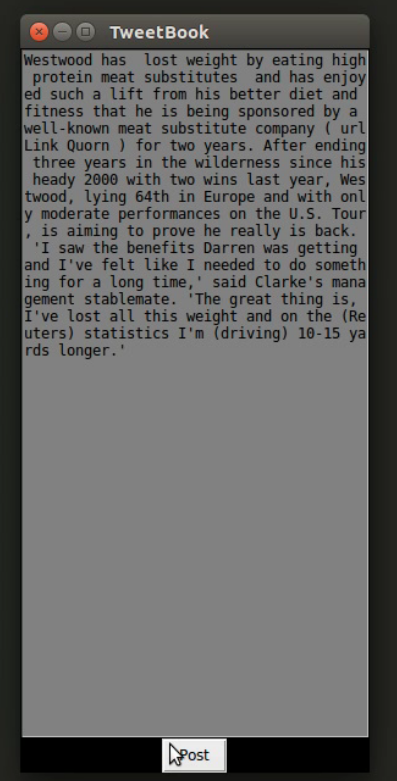
\includegraphics[width=50mm]{./Images/demo2}
%  \caption{Attempting to send a post that belongs to the authorized user.}
%  \label{demo2}
%\end{figure}
%
%\begin{figure}[h]
%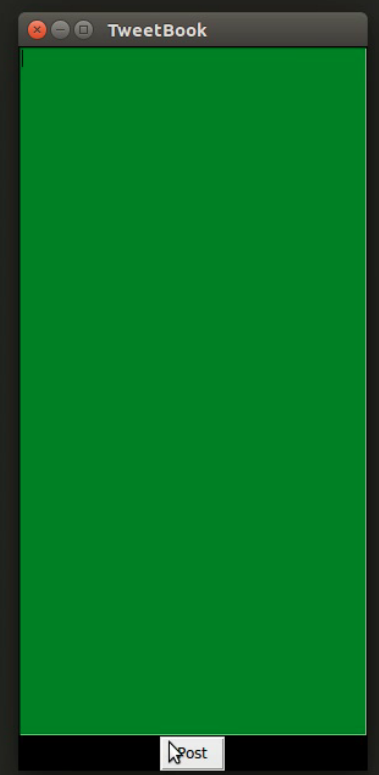
\includegraphics[width=50mm]{./Images/demo3}
%  \caption{The post belonging to the authorized user was sent successfully.}
%  \label{demo3}
%\end{figure}
%
%\begin{figure}[h]
%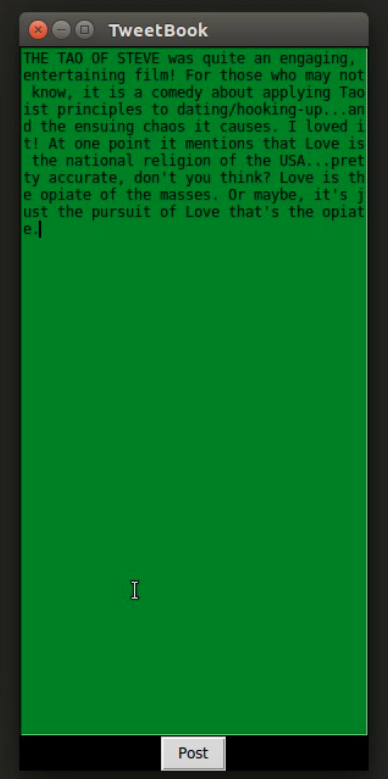
\includegraphics[width=50mm]{./Images/demo4}
%  \caption{Attempting to send a post that does not belong to the authorized user.}
%  \label{demo4}
%\end{figure}
%
%\begin{figure}[h]
%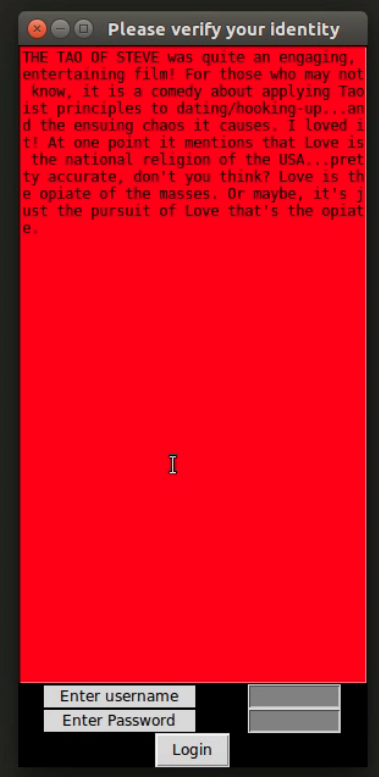
\includegraphics[width=50mm]{./Images/demo5}
%  \caption{The post that does not belong to the authorized user failed to send and the user was locked out of the social media application until they can verify that they are the authorized user.}
%  \label{demo5}
%\end{figure}



%\section{Code for demonstration}
%\begin{figure}
%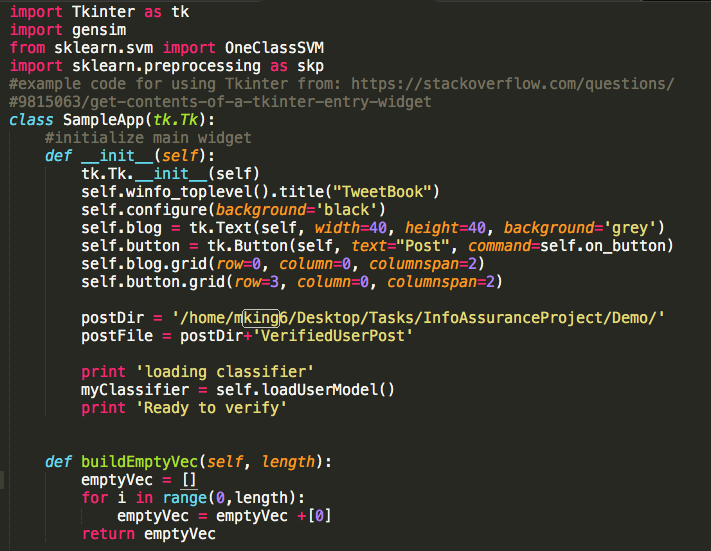
\includegraphics[width=\linewidth]{./Images/demoCode1}
%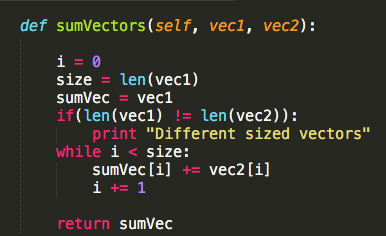
\includegraphics[width=\linewidth]{./Images/demoCode2}
%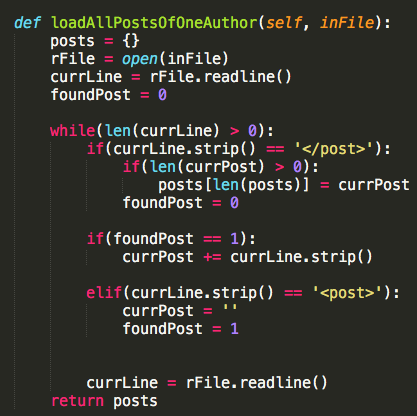
\includegraphics[width=\linewidth]{./Images/demoCode3}
%  \caption{First half of the python code for the demonstration.}
%  \label{demoCode1}
%\end{figure}

%\begin{figure}

%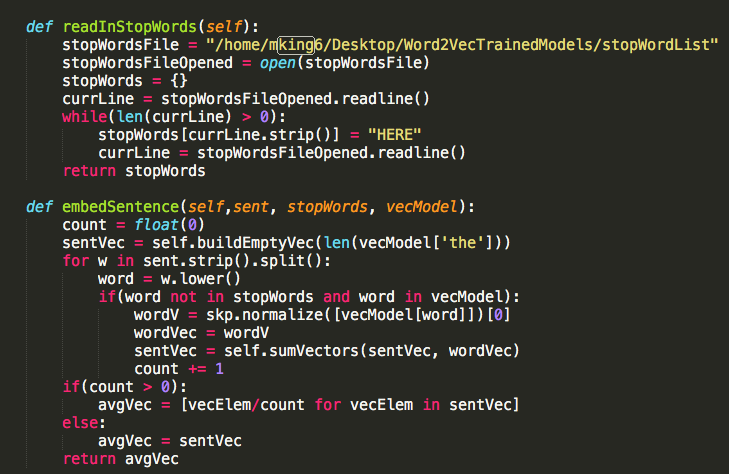
\includegraphics[width=\linewidth]{./Images/demoCode4}
%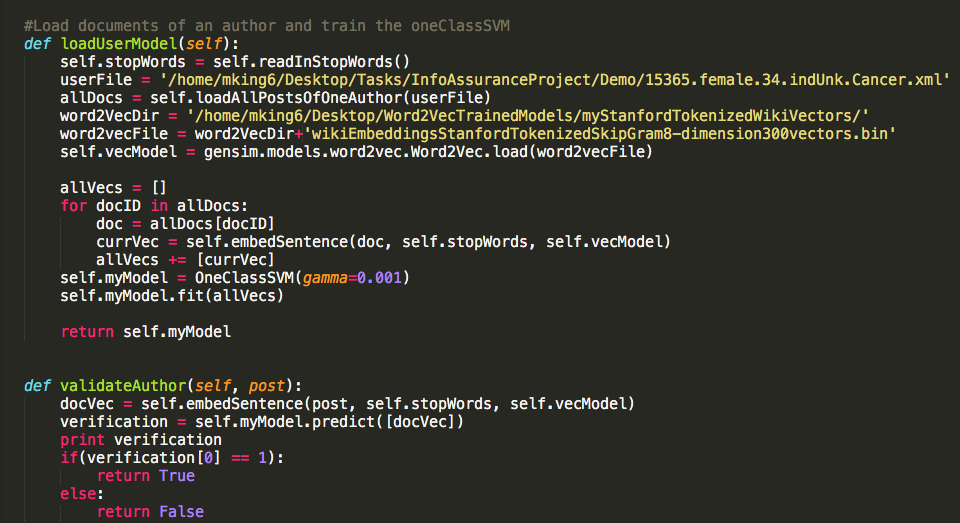
\includegraphics[width=\linewidth]{./Images/demoCode5}
%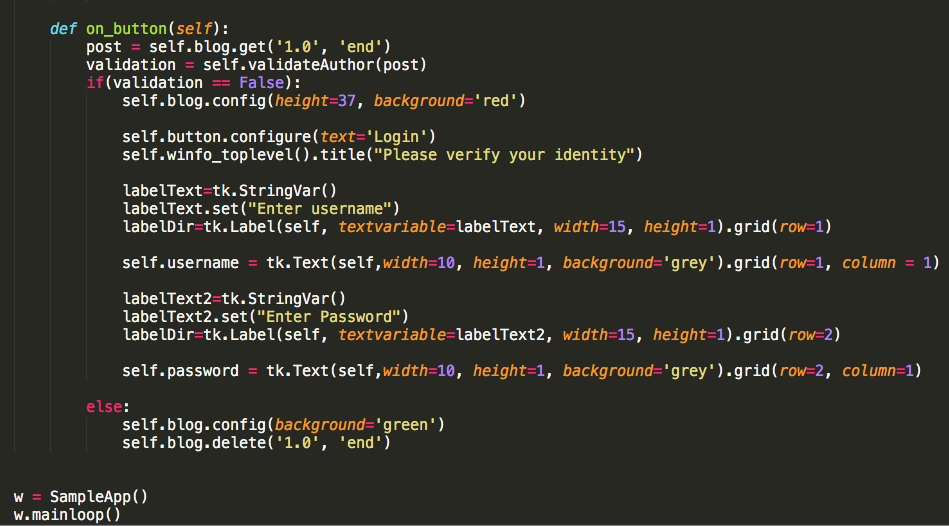
\includegraphics[width=\linewidth]{./Images/demoCode6}
%  \caption{Second half of the python code for the demonstration}
%  \label{demoCode2}
%\end{figure}


%%%%IDEAS for trimming
%Reduce introduction Check
%Reduce related work Check
%When discussing PAN models try to cite only the task overview paper
%provide url to scikit learn instead of refrence Check
%Remove DEV tuning tables and just mentioned that we tuned to this Check
%Reduce discussion in Experimental results seciton. Do not trim if there is interesting material
%Remove figure 1 and 2 but can mention them for motivation (Keep one exmaple, the financial one)
%Make more clear about choosing the threshold
%Make clear that we use cosine in order to work with vectors
%Add a second paper that used stopwords
%Discuss Wikipedia
%Emphasize more why we didn't choose the PAN dataset
%Check footnotes are before or after period

\end{document}



